% Options for packages loaded elsewhere
\PassOptionsToPackage{unicode}{hyperref}
\PassOptionsToPackage{hyphens}{url}
%
\documentclass[
]{article}
\usepackage{lmodern}
\usepackage{amssymb,amsmath}
\usepackage{ifxetex,ifluatex}
\ifnum 0\ifxetex 1\fi\ifluatex 1\fi=0 % if pdftex
  \usepackage[T1]{fontenc}
  \usepackage[utf8]{inputenc}
  \usepackage{textcomp} % provide euro and other symbols
\else % if luatex or xetex
  \usepackage{unicode-math}
  \defaultfontfeatures{Scale=MatchLowercase}
  \defaultfontfeatures[\rmfamily]{Ligatures=TeX,Scale=1}
\fi
% Use upquote if available, for straight quotes in verbatim environments
\IfFileExists{upquote.sty}{\usepackage{upquote}}{}
\IfFileExists{microtype.sty}{% use microtype if available
  \usepackage[]{microtype}
  \UseMicrotypeSet[protrusion]{basicmath} % disable protrusion for tt fonts
}{}
\makeatletter
\@ifundefined{KOMAClassName}{% if non-KOMA class
  \IfFileExists{parskip.sty}{%
    \usepackage{parskip}
  }{% else
    \setlength{\parindent}{0pt}
    \setlength{\parskip}{6pt plus 2pt minus 1pt}}
}{% if KOMA class
  \KOMAoptions{parskip=half}}
\makeatother
\usepackage{xcolor}
\IfFileExists{xurl.sty}{\usepackage{xurl}}{} % add URL line breaks if available
\IfFileExists{bookmark.sty}{\usepackage{bookmark}}{\usepackage{hyperref}}
\hypersetup{
  pdftitle={Laboratorio: Planificación STRIPS},
  pdfauthor={Richard Camilo Saavedra Coneo},
  hidelinks,
  pdfcreator={LaTeX via pandoc}}
\urlstyle{same} % disable monospaced font for URLs
\usepackage[margin=1in]{geometry}
\usepackage{graphicx,grffile}
\makeatletter
\def\maxwidth{\ifdim\Gin@nat@width>\linewidth\linewidth\else\Gin@nat@width\fi}
\def\maxheight{\ifdim\Gin@nat@height>\textheight\textheight\else\Gin@nat@height\fi}
\makeatother
% Scale images if necessary, so that they will not overflow the page
% margins by default, and it is still possible to overwrite the defaults
% using explicit options in \includegraphics[width, height, ...]{}
\setkeys{Gin}{width=\maxwidth,height=\maxheight,keepaspectratio}
% Set default figure placement to htbp
\makeatletter
\def\fps@figure{htbp}
\makeatother
\setlength{\emergencystretch}{3em} % prevent overfull lines
\providecommand{\tightlist}{%
  \setlength{\itemsep}{0pt}\setlength{\parskip}{0pt}}
\setcounter{secnumdepth}{-\maxdimen} % remove section numbering

\title{Laboratorio: Planificación STRIPS}
\author{Richard Camilo Saavedra Coneo}
\date{24/6/2020}

\begin{document}
\maketitle

\hypertarget{descripciuxf3n-de-la-actividad}{%
\paragraph{Descripción de la
actividad:}\label{descripciuxf3n-de-la-actividad}}

Expresa el siguiente escenario en la representación tipo STRIPS:

En una habitación hay un mono, una caja y un plátano, tal como indica la
figura (situación inicial). El objetivo del mono es tener el plátano. El
mono puede:

\begin{itemize}
\tightlist
\item
  Ir de una posición a otra.
\item
  Empujar la caja de una posición a otra si está en la misma posición
  que ella no está sobre ella.
\item
  Subirse a la caja si está en la misma posición que ella.
\item
  Coger el plátano si está en encima de la caja.
\end{itemize}

\begin{figure}
\centering
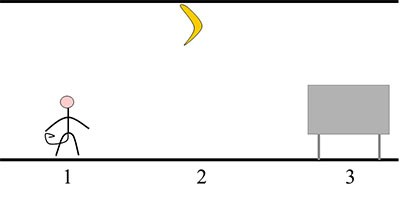
\includegraphics{https://github.com/richardcmg7/pddl/blob/master/img/img1.jpg?raw=true}
\caption{Imagen Representación}
\end{figure}

Modelar en PDDL (dominio.pddl y problema{[}S{]}.pddl - 3 problemas) el
mismo escenario que se plantea en la actividad y resolver los problemas
con 3 planificadores del estado del arte.

\end{document}
